%%%  本笔记完全参考morelulll.cls
\documentclass[UTF8, twoside, fontset=none]{ctexart}

%%% 宏
\usepackage[headheight=127mm, left=2cm, right=2cm, bottom=2cm]{geometry}    % headheight过小不被允许故设置了一个下限
% % \geometry{}	paper=a4paper, % Change to letterpaper for US letter
% 	inner=2.5cm, % Inner margin
% 	outer=3.8cm, % Outer margin
% 	bindingoffset=.5cm, % Binding offset
% 	top=1.5cm, % Top margin
% 	bottom=1.5cm, % Bottom margin
% 	%showframe, % Uncomment to show how the type block is set on the page


%%% 字体设置 %%%
\usepackage[T1]{fontenc}
\usepackage{textcomp}  % for \textquotesingle macro
% 英文等宽字体
% \setmonofont{Fantasque Sans Mono}
\usepackage{xeCJK}
\setCJKmainfont{simsun.ttc}
% \setCJKsansfont{}
\setCJKmonofont{simfang.ttf}
% \setCJKmainfont{方正书宋_GBK}
% \setCJKsansfont{方正书宋_GBK}
% 只有方正字体支持CJK脚本(CJK Script)
\setCJKfamilyfont{zhhei}{simhei.ttf}[BoldFont=simhei.ttf, ItalicFont=fantasquesansmono-bolditalic.otf]
\setCJKfamilyfont{zhyou}{FZY1K.TTF}[BoldFont=FZY1K.TTF, ItalicFont=FZY3K.TTF]
\setCJKfamilyfont{方正楷体}{FZKTJW.TTF}
% 由于为了使用上述CJK宏的主要字族/无衬线字族/有衬线字族
% 字体需要确定到本地windows文件夹Fonts子文件夹的字体名称
% LaTeX的字体逻辑 字族\字体\字形
% 由于使用fontset=none的ctexart文类需要重新定义\heiti \songti \kaishu等命令
\newcommand{\heiti}[1]{{\CJKfamily{zhhei}{#1}}}
\newcommand{\youyuan}[1]{{\CJKfamily{zhyou}{#1}}}

%%% 链接设置
% 定义颜色
\usepackage{xcolor}
\definecolor{DarkRed}{RGB}{139,0,0}
\definecolor{DimGrey}{RGB}{105 105 105}
\definecolor{ShallowGray}{RGB}{220, 220, 220}
\definecolor{CommentGreen}{RGB}{0, 255, 0}
\definecolor{KeyMauve}{RGB}{204, 153, 255}
\definecolor{thmcolor}{RGB}{241, 241, 255}
\definecolor{defcolor}{RGB}{100, 149, 237}
% 超链接设置
\usepackage[
    colorlinks=true,
    linkcolor=DarkRed,
    linkbordercolor=DarkRed,
    anchorcolor=DimGrey,
    citecolor=DarkRed,
    plainpages=false,
    pdfencoding=unicode,
    hypertexnames=true,
]{hyperref}
% 定理环境
\usepackage{amsmath,amssymb,amsthm,amsfonts}
\usepackage{mathtools}      % 数学符号美化
\usepackage{tikz-cd}
\usepackage{verbatim}       % 注释
\allowdisplaybreaks[4]      % 公式跨页
\renewcommand\theequation{\thetheorem\alph{equation}}
\newtheorem{theorem}{定理}[section]
\newtheorem{proposition}[theorem]{\heiti{命题}}
\newtheorem{corollary}{\youyuan{推论}}[theorem]
\newtheorem{lemma}{\youyuan{引理}}[theorem]
\newtheorem{definition}{$\blacksquare$ \,定义}[section]

%%% 页眉页脚设置
\usepackage{fancyhdr}
\pagestyle{fancy}
\fancyhead[C]{\textcolor{black}{\leftmark}}
\fancyhead[RO,LE]{\textcolor{DimGrey}{\thepage}}
\fancyhead[RE,LO]{}
\fancyfoot{}
\renewcommand{\headrule}{\color{DimGrey}\hrule width\textwidth}

%   文本提示
\usepackage{tcolorbox}
\tcbuselibrary{breakable,skins}
\tcbsetforeverylayer{enhanced}
\newtcolorbox[auto counter,number within=section]{notebox}[1]{
    skin=empty,
    top = 0pt,
    bottom = 0pt,
    toprule = 0pt,
    bottomrule = 0pt,
    leftrule = 0pt,
    rightrule = 0pt,
    borderline west={2pt}{0pt}{#1},
    breakable, %允许跨页
}

% 注
\newenvironment{note}
{\begin{notebox}{orange}
      \textcolor{orange}{ \CJKfamily{zhhei}{注:}}
}
{\end{notebox}}

% 例
\newenvironment{case}
{\begin{notebox}{blue}
      \textcolor{blue}{ \CJKfamily{zhhei}{例:}}
}
{\end{notebox}}

% 论断
\newtcolorbox{claim}{colframe = blue!75!black}

% 引用结论
\renewenvironment{quote}
{\begin{notebox}{gray}
      \textcolor{gray}{ \CJKfamily{zhhei}{\textbullet}}
}
{\end{notebox}}

%%% 参考文献配置
\usepackage[backend=biber,backref=true,bibstyle=draft,citestyle=ext-authoryear]{biblatex}
\DeclareOuterCiteDelims{cite}{\bibopenbracket}{\bibclosebracket}
\AtEveryCite{\color{blue}}      %   蓝色引用文字
\addbibresource{HUAWEI_Linghang.bib}



%%% 命令简化
\renewcommand{\O}{\mathcal{O}}
\renewcommand{\contentsname}{\heiti{论文目录}}  %   重新设置目录标题



%%% 文件树呈现
\usepackage{forest}



%%% 代码解释
\usepackage{listings}
\lstset{ %
  backgroundcolor=\color{ShallowGray},      % choose the background color
  basicstyle=\footnotesize,                 % size of fonts used for the code
  breaklines=true,                          % automatic line breaking only at whitespace
  captionpos=b,                             % sets the caption-position to bottom
  commentstyle=\color{CommentGreen},        % comment style
%   escapeinside={\%*}{*)},                 % if you want to add LaTeX within your code
  keywordstyle=\color{blue},                % keyword style
  stringstyle=\color{KeyMauve},             % string literal style
  frame=single,
  numbers=left,
}



%%% 扉页设置
%   预定义命令
\NewDocumentCommand{\thesistitle}{ o m }{
    \IfValueTF{#1}{\def\shorttitle{#1}}{\def\shorttitle{#2}}
    \def\@title{#2}
    \def\ttitle{#2}
    }
% \DeclareDocumentCommand{\author}{m}{\newcommand{\authorname}{#1}\renewcommand{\@author}{#1}}
\NewDocumentCommand{\supervisor}{m}{\newcommand{\supname}{#1}}
\NewDocumentCommand{\examiner}{m}{\newcommand{\examname}{#1}}
\NewDocumentCommand{\degree}{m}{\newcommand{\degreename}{#1}}
\NewDocumentCommand{\addresses}{m}{\newcommand{\addressname}{#1}}
\NewDocumentCommand{\university}{m}{\newcommand{\univname}{#1}}
\NewDocumentCommand{\department}{m}{\newcommand{\deptname}{#1}}
\NewDocumentCommand{\group}{m}{\newcommand{\groupname}{#1}}
\NewDocumentCommand{\faculty}{m}{\newcommand{\facname}{#1}}
\NewDocumentCommand{\subject}{m}{\newcommand{\subjectname}{#1}}
\NewDocumentCommand{\keywords}{m}{\newcommand{\keywordnames}{#1}}
\newcommand{\HRule}{\rule{.9\linewidth}{.6pt}} % New command to make the lines in the title page
%	论文信息
\thesistitle{Low Dissipation and Adaptive FIR Filter Algorithms} % Your thesis title, this is used in the title and abstract, print it elsewhere with \ttitle
\supervisor{\textsc{REK3000}} % Your supervisor's name, this is used in the title page, print it elsewhere with \supname
\examiner{} % Your examiner's name, this is not currently used anywhere in the template, print it elsewhere with \examname
\degree{HUAWEI Applied Mathematics Contest} % Your degree name, this is used in the title page and abstract, print it elsewhere with \degreename
\addresses{Shanghai,China} % Your address, this is not currently used anywhere in the template, print it elsewhere with \addressname
\subject{Hardware Algorithms} % Your subject area, this is not currently used anywhere in the template, print it elsewhere with \subjectname
\keywords{} % Keywords for your thesis, this is not currently used anywhere in the template, print it elsewhere with \keywordnames
\university{\href{https://yotally.github.io/}{HUAWEI APPLIED MATHEMATICAL CONTEST}} % Your university's name and URL, this is used in the title page and abstract, print it elsewhere with \univname
\department{\href{null}{Chai Hao in SMCS,Fudan University,\\
Li Minghao in EIE,Nanjiing University,\\
Wang Xiyuan in SMS,Fudan University}} % Your department's name and URL, this is used in the title page and abstract, print it elsewhere with \deptname
\group{\href{https://yotally.github.io/}{Fudan University, Nanjing University}} % Your research group's name and URL, this is used in the title page, print it elsewhere with \groupname
\faculty{\href{https://github.com/YOTALTEAM}{REK3000}} % Your faculty's name and URL, this is used in the title page and abstract, print it elsewhere with \facname
%   文档起始设置超链接格式
\AtBeginDocument{
	\hypersetup{pdftitle=\ttitle} % Set the PDF's title to your title
    % \hypersetup{pdfauthor=\authorname} % Set the PDF's author to your name
	\hypersetup{pdfkeywords=\keywordnames} % Set the PDF's keywords to your keywords
	\hypersetup{hypertexnames=true} % Make bib index back reference a right position
}

\title{ \heiti{华为领航杯应用数学大赛论文}\\
低功耗自适应有限脉冲滤波器算法}

\author{} % Your name, this is used in the title page and abstract, print it elsewhere with \authorname

\date{2023.8}

\begin{document}

% \frontmatter % Use roman page numbering style (i, ii, iii, iv...) for the pre-content pages

\pagestyle{plain} % Default to the plain heading style until the thesis style is called for the body content

%----------------------------------------------------------------------------------------
%	TITLE PAGE
%----------------------------------------------------------------------------------------

\begin{titlepage}
    \begin{center}
    
    \vspace*{.06\textheight}
    {\scshape\LARGE \univname\par}\vspace{1.5cm} % University name
    \textsc{\Large Contest Thesis}\\[0.5cm] % Thesis type
    
    \HRule \\[0.4cm] % Horizontal line
    {\LARGE \bfseries \ttitle\par}\vspace{0.4cm} % Thesis title
    \HRule \\[1.5cm] % Horizontal line
     
    \begin{minipage}[t]{0.4\textwidth}
    \begin{flushleft} \large
    \emph{Author:}\\
    \href{https://github.com/YOTALTEAM}{Chai Hao, \\
                                    Li Minghao, \\
                                    Wang Xiyuan} % Author name (remove the \href bracket to remove the link)
    \end{flushleft}
    \end{minipage}
    \begin{minipage}[t]{0.4\textwidth}
    \begin{flushright} \large
    \emph{Team:} \\
    \href{https://github.com/YOTALTEAM}{\supname} % Supervisor name - remove the \href bracket to remove the link  
    \end{flushright}
    \end{minipage}\\[3cm]
     
    \vfill
    
    \large \textit{A thesis submitted in fulfillment of the requirements\\ for the \degreename Applied Mathematics Contest}\\[0.3cm] % University requirement text
    \textit{in August 2023}\\[0.4cm]
    \groupname \\ \deptname \\[2cm] % Research group name and department name
     
    \vfill
    \end{center}
\end{titlepage}

\maketitle

\begin{abstract}
    本文主要实现一种低功耗(Low Dissipation)自适应(Adaptive)的有限长单位脉冲响应滤波器(Finite Impulse 
    Response Filter)算法。主要参考文献是 \cite{Winograd1968,Gholami2021,Jiang2020,Cormen2022,Nussbaumer1982}。

    低功耗算法的主要思想是两类:一是等价改变滤波器架构最小化乘法器个数;二是降低滤波器的乘法器的运算复杂度。其中
    架构的不同实现包含 Cooley-Tukey 算法、内积加速算法\cite{Winograd1968}、Karatsuba 快乘\cite{Karatsuba1995}
    (主要是通过减少乘法而加速离散傅立叶变换,通论可见快速\cite[Chap1,2]{Nussbaumer1982});加速乘法器本身的算法诸如
    tooth加速乘法\cite{Li2010}、近似乘法和量化感知优化\cite{Gholami2021}(中文写成的数值计算神书
    \cite{Li2010}有详尽说明)。

    自适应算法采用机器学习预测算法,主要保证快速校正和模型无损(题目的诉求三)。通过预测信号量进行自适应滤波能够输出指定的
    或期望的样式信号,以达到降噪、降低功耗、快速响应等实时场景的不同要求。
    
    本文是第一届华为领航杯应用数学大赛参数论文。本文之格式内容均依照该竞赛要求完成。
\end{abstract}

\newpage 

%   目录标题颜色
{\color{DarkRed}\tableofcontents}

\newpage

\clearpage

% \mainmatter % Begin numeric (1,2,3...) page numbering

\section{问题背景阐述}

\subsection{回顾极坐标下黎曼度量}

简扼讲黎曼流形 $(M,g)$ 是一个光滑流形上带有对称的度量 $g \in \mathrm{Sym}_2(TM) \subset T^*M \otimes T^*M $ 。现在考虑局部坐标 $(x^i)_i$
和 $(y^i)_i$ 以及其坐标变换 $F:(x^i)_i \to (y^i)_i$ 的Fr\'echet导数 $D_F = (\frac{\partial y^i}{\partial x^j})_ij$。在两个坐标下度量有不同形式
\begin{equation*}
    g  = g_{ij} dx^i dx^j = \tilde{g}_{kl}dy^k dy^l = g_{ij}\frac{\partial x^i}{\partial y^k}\frac{\partial x^j}{\partial y^l}d y^k dy^l
\end{equation*}
沿袭Einstein求和约定(相同指标代表求和)利用唯一性可知 $\tilde{g}_{kl} = g_{ij}\frac{\partial x^i}{\partial y^k}\frac{\partial x^j}{\partial y^l}$
记 $G = (g_{ij})_{ij}$ 为度量矩阵而 $G^{-1} = (g^{ij})_{ij}$ 为其逆可知 $\tilde{G} = (\tilde{g}_{ij})_{ij} = D_{F^{-1}}^{t}G D_{F^{-1}}$。
再次利用Fr\'echet导数和切映射的联系
\begin{equation*}
    D_F D_{F^{-1}} = I_n,\quad n = \dim M, \quad 
\end{equation*} 
从而体积元 $dV_g = \sqrt{|det G_x|} dx^1\wedge\cdots\wedge d x^n $ 具有协变性(在 $F$ 保定向的情况下此时 $\det D_F >0$)
\begin{align*}
    &dV_g = \sqrt{|det G|} dx^1\wedge\cdots\wedge d x^n \tag*{(V1)}\\
    &d\widetilde{V_g} = \sqrt{|det \tilde{G}|} dy^1\wedge\cdots\wedge d y^n\\
    &d\widetilde{V_g}  =  \sqrt{|det G|} |\det D_F|^{-1} |\det D_F| dx^1\wedge\cdots\wedge d x^n  = \sqrt{|det G|} dx^1\wedge\cdots\wedge d x^n = dV_g
\end{align*}
协变性表示公式形式不依赖于坐标选择,从而 $dV_g$ 是一个内蕴的几何量只和度量 $g$ 有关。
对于流形上的函数 $f \in C^\infty(M)$ 定义其梯度是内蕴量
\begin{equation*}
    \langle \nabla f, X \rangle_g = X(f),\quad forall X \in X(M)
\end{equation*}
代入坐标即 $g_{ij}(\nabla f)^i X^j = \sum_i X^i\partial_i f$ 有 $(\nabla f)^i = \partial^i f = g^{ij}\partial_j f$。这个梯度公式是协变的
一方面可以从其定义的内蕴性得到另一方面可以直接计算

下面为了求和规则记 $\partial_i = \frac{\partial}{\partial x^i},\tilde{\partial}_i = \frac{\partial}{\partial y^i}$ 或者用合适下标表示
偏导变量类如 $\partial_{x,i}$ 等
\begin{align*}
    \tilde{g}^{ij}\tilde{\partial}_j f \tilde{\partial}_i & = \partial_k y_i g^{kl} \partial_l y_j \partial_m f \tilde{\partial}_{j}x^m \tilde{\partial}_i x^n \partial_n \\
                & = g^{kl}\partial_m f \partial_n  (\partial_k y_i \tilde{\partial}_i x^n ) (\partial_l y_j \tilde{\partial}_{j}x^m )\\
                & =  \delta_{kn} \delta_{lm} g^{kl}\partial_m f \partial_n = g^{ij}\partial_j f \partial_i 
\end{align*}

$\nabla f = \mathrm{grad} f $ 具有协变公式 $\nabla f = g^{ij}\partial_j f \partial_i $。次考虑切向量场 $X(M)$
的散度 $\mathrm{div} X$ 其可以内蕴地定义为
\begin{equation*}
    d (X \mathrel{\lrcorner} dV_g) = (\nabla X) dV_g
\end{equation*}
利用李导数的Cartan公式和 $d (dV_g) = 0$ 也可得到 $L_X (dV_g) = d (\iota_X (dV_g)) = \iota_X(d(dV_g)) =  d (X \mathrel{\lrcorner} dV_g)  = (\nabla X) dV_g$

这里 $X \lrcorner dV_g = \iota_X (dV_g)$ 是切向量场的缩并运算。

简记 $|g| = |\det G|$ 表示黎曼测度的体积膨胀性质。显式计算出
\begin{align*}
    \nabla \cdot X = \mathrm{div} X & = \star (\frac{1}{\sqrt{|g|}} d(\sum_i \sqrt{|g|}X^i(-1)^{i-1}dx^1\wedge \cdots \wedge \widehat{dx^i} \wedge \cdots \wedge dx^n))\\
    & = \star (\frac{1}{\sqrt{|g|}} \partial_i (\sqrt{|g|}X^i) dV_g)\\
    & = \frac{1}{\sqrt{|g|}} \partial_i (\sqrt{|g|}X^i)
\end{align*}
可以直接计算上述公式的内蕴性质,只需要利用矩阵微积分中的性质
\begin{align*}
    &\frac{d}{dt}\det A(t) = \Tr(A^{adj}(t)\frac{dA(t)}{dt}) = \det(A) \Tr (A^{-1}(t)\frac{dA(t)}{dt})\\
    &\frac{d}{dt} \ln |\det A(t)| \frac{1}{\det A(t)} \frac{d}{dt}\det A(t) = \Tr (A^{-1}(t)\frac{dA(t)}{dt}) \tag*{(A1)}
\end{align*}
上述关系称为Jacobi Formula。本质来自于矩阵群 $\mathrm{M}_n(\C)$ 的切向量满足 $\nabla_{T}\det (I_n)= \Tr T$ 从而计算记 $H = F^{-1}$
\begin{align*}
    \nabla  X 
    & = \frac{1}{\sqrt{|\tilde{g}|}} \tilde{\partial}_k (\sqrt{|\tilde{g}|}Y^k) = \frac{1}{|\det D_H|} \frac{1}{\sqrt{|g|}} \tilde{\partial}_k x^i \partial_i (\sqrt{|g|}|\det D_H|\partial_j y^k X^j)\\
    & = \frac{1}{\sqrt{|g|}} \partial_i (\sqrt{|g|}X^j) \partial_j y^k \tilde{\partial}_k x^i + X^i (\partial_i \ln |\det D_H| + \tilde{\partial}_k x^j \partial_{ij} y^k)\\
    & = \frac{1}{\sqrt{|g|}} \partial_i (\sqrt{|g|}X^j) \delta_{ij} + X^i (\Tr(D_F (\partial_i D_H) )+ \tilde{\partial}_k x^j \partial_{ij} y^k) \,\quad  \text{利用矩阵微积分A1}\\
    & = \frac{1}{\sqrt{|g|}} \partial_i (\sqrt{|g|}X^j) + X^i(\partial_k y^j \partial_i (\tilde{\partial}_j x^k) + \tilde{\partial}_j x^k \partial_i (\partial_k y^j)) \quad \text{展开} \\
    & = \frac{1}{\sqrt{|g|}} \partial_i (\sqrt{|g|}X^j) + X^i \partial_i (\partial_k y^j \tilde{\partial}_j x^k),\quad \text{莱布尼兹法则}\\
    & =  \frac{1}{\sqrt{|g|}} \partial_i (\sqrt{|g|}X^j) + X^i \partial_i(\dim M) =  \frac{1}{\sqrt{|g|}} \partial_i (\sqrt{|g|}X^j) \tag*{(A2)}
\end{align*}
从而说明了散度公式的协变性。

从梯度和散度出发,对于函数 $f \in C^\infty (M)$ 定义Laplace-Beltrami算子是两者复合
\begin{equation*}
    \Delta_g f  := \mathrm{div} \circ \mathrm{grad}f
\end{equation*}
写成协变的形式就是
\begin{equation*}
    \Delta_g f := \frac{1}{\sqrt{|g|}} \partial_i (\sqrt{|g|}g^{ij}\partial_j f )
\end{equation*}
根据梯度和散点的协变性可知 $\Delta_g f$ 不依赖于坐标选择,事实上算子
\begin{equation*}
    \Delta_g := \frac{1}{\sqrt{|g|}} \partial_i (\sqrt{|g|}g^{ij}\partial_j ) \quad \tag*{(V3)}
\end{equation*}
也是协变的,只需类似验证散点的协变性计算。

利用 $\tilde{g}^{ij} \tilde{\partial}_j = \partial_j y^i( g^{jk} {\partial}_k)$ 如果取 
$Y^i = \tilde{g}^{ij} \tilde{\partial}_j $ 和 $X^i = g^{ij}{\partial}_j $ 则自然满足协变性 $Y^i = \partial_j y^i X^j$。这
正是切向量的坐标变换方式,代入在(A2) 中的计算可知
\begin{align*}
    \widetilde{\Delta_g} &= \frac{1}{\sqrt{\tilde{g}|}} \tilde{\partial}_i (\sqrt{|\tilde{g}|}\tilde{g}^{ij}\tilde{\partial}_j ) = \frac{1}{\sqrt{|\tilde{g}|}} \tilde{\partial}_k (\sqrt{|\tilde{g}|}Y^k)\\
    & = \frac{1}{\sqrt{|g|}} \partial_i (\sqrt{|g|}X^i ) =  \frac{1}{\sqrt{|g|}} \partial_i (\sqrt{|g|}g^{ij}\partial_j )
\end{align*}
就得到了Laplace-Beltrami算子的协变性。

对于典范的黎曼模型 $(M,g)$ 其度规在标准坐标下是 $g = g_ij dx^i dx^j$ 换算成极坐标$(r,\theta)$下可以写成
\begin{align*}
    &g_M := dr^2 + \psi(r)^2 g_{\mathbb{S}^{n-1}},\quad\\
    &g_{\mathbb{S}^{n-1}} = \langle \nabla_{\theta}\frac{x}{r},\nabla_{\theta}\frac{x}{r}\rangle
    = (\sum_k\partial_{\theta_i}(\frac{x_k}{r})\partial_{\theta_j}(\frac{x_k}{r}))d\theta^i d\theta^j
    = \gamma_{ij}d\theta^i d\theta^j \\
    &\text{是球面的标准欧式度量}
\end{align*}
那么可以计算出 $(M,g)$ 的体积形式,其不依赖于坐标,选择极坐标 $(r,\theta)$ 其度量矩阵形如
\begin{equation*}
    G = 
    \left(
        \begin{matrix}
            1   & \\
                &\psi^{2}(r)G_{\mathbb{S}^{n-1}}\\
        \end{matrix}
    \right),\quad G^{-1} = 
    \left(
        \begin{matrix}
            1   & \\
                &\psi^{-2}(r)G_{\mathbb{S}^{n-1}}^{-1}\\
        \end{matrix}
    \right)
\end{equation*}
从而利用上述的内蕴公式(V1)计算出此时
\begin{equation*}
    d \nu = dV_g = \sqrt{|\det G|}dr \wedge d\theta = \psi^{n-1}(r)dr \wedge (\sqrt{|\det G_{\mathbb{S}^{n-1}}}|d\theta) = \psi^{n-1}(r)dr \wedge d \sigma_{\mathbb{S}^{n-1}}
\end{equation*}
其中 $d \sigma_{\mathbb{S}^{n-1}} = \sqrt{|\det g_{\mathbb{S}^{n-1}|}}d\theta$ 是标准球面的黎曼测度。另外利用此矩阵结构计算极坐标下的
Laplace算子利用协变公式(V3)可以得到
\begin{equation*}
    \Delta_g := \frac{1}{\sqrt{|g|}} \partial_i (\sqrt{|g|}g^{ij}\partial_j )
    =     \frac{\partial_r (\psi^{n-1} |g_{\mathbb{S}^{n-1}}| \partial_r)}{\psi^{n-1} |g_{\mathbb{S}^{n-1}}|}  
    + \frac{\partial_{\theta_i} ( \psi^{n-1} \psi^{-2} g_{\mathbb{S}^{n-1}}^{ij} \partial_{\theta_j})}{\psi^{n-1} |g_{\mathbb{S}^{n-1}}|}
    = \frac{1}{\psi^{n-1}}\partial_r (\psi^{n-1}\partial_r) + \frac{1}{\psi^2}\Delta_{\mathbb{S}^{n-1}}
\end{equation*}
也就是
\begin{equation*}
    \Delta_g := \frac{\partial^2}{\partial r^2} + \frac{\partial }{\partial r}(\ln \psi^{n-1}(r)) \frac{\partial }{\partial r} + \frac{1}{\psi^2(r)}\Delta_{\mathbb{S}^{n-1}}
\end{equation*}


\subsection{李导数和流形上的李代数}


\subsection{流形积分和Hodge对偶}


\section{经典方法复现}


\section{\heiti{理论及算法}}

\subsection{\heiti{离散傅立叶变换(Discrete Fourier Transformatioin, FFT) 的快速实现}}

基于第二部分经典理论,本项目实现高精度 FFT 流处理器的主要方式如下所述。
\paragraph{\heiti{高性能 FFT 流处理器:基于冗余计算和折叠架构的浮点运算蝶形阵列}}
为实现小面积、高并行、高灵活度的 FFT 处理单元,本文创新性地提出了FFT流处理器,通过冗余计算和架构折叠来取得面积和运算效率的最佳权衡。

该部分创新点可总结为:
\begin{itemize}
    \item   基于冗余计算提出了具有极短关键路径的``冗余串行乘法''单元和``冗余浮点加法单元'',
    他们的关键路径仅有 $2$ 到 $3$ 个全加器(Full Adder,FA)。
    \item   通过乘加运算折叠(Folding)使得浮点数运算的复杂度极限接近定点数运算。
    \item   通过蝶形单元展开(Unfolding)使得选用各层同性FFT拓扑成为可能,从而充分简化系统控制逻辑,减少硬件运算单元在处理数据中的等待和空拍,提高硬件资源利用率。
    \item   依赖于数据的冗余表示法和各层同性的 FFT 拓扑,实现了紧凑的数据流映射方案。
    \item   使得系统的面积效率获得较大提升。
    \item   具体而言:(1)通过折叠乘加运算;(2)通过扩大蝶形单元并行度。
\end{itemize}

总结而言,在设计策略上,本文通过冗余计算使得浮点数乘、加运算取得较好的架构折叠方案;进一步通过灵活应用折叠和展开技术,实现了在相同面积约束下
,乘、加子运算并行度与蝶形单元个数(FFT处理点数并行度)之间的权衡,从而取得较为理想的面积效率。

此外更加高效的办法是参考 \cite{Li2010}。或者关于快速傅立叶变换的综述性质书籍\cite{Nussbaumer1982}。

\paragraph{\heiti{基于冗余计算的折叠蝶形计算阵列}}
图\ref{fig:Float-Redundant-Butterfly-Unit} 所示 Butterfly Unit 完成 FFT 所需的蝶形运算即
\begin{eqnarray*}
    \left\{
        \begin{aligned}
        E=Y+R\cdot X\\
        F=Y-R\cdot X
        \end{aligned}
        \right.
\end{eqnarray*}

而完成一个蝶形运算共需要两级流水线:
\begin{itemize}
    \item \heiti{第一级流水线}为冗余乘法:FFT上一级蝶形运算的输出,
            经过 Mapping 拓扑映射单元送往当前蝶形运算的输入端,
            随着输入数据的串入,乘法执行结束,与次同时,
            乘法器的输出也逐个数位地输入到 Aligning Buffer 中,
            便于后续冗余加、减法操作;
    \item \heiti{第二级流水线}为冗余浮点加、减法:
            从 Aligning Buffer 先后输出的数据被加、减归约,
            其输出被送往 Mapping 单元,以便输送给 FFT 下一级蝶形运算对应蝶形结的输入端。
\end{itemize}


\begin{center}
    \begin{figure}[ht!]
        \centering
        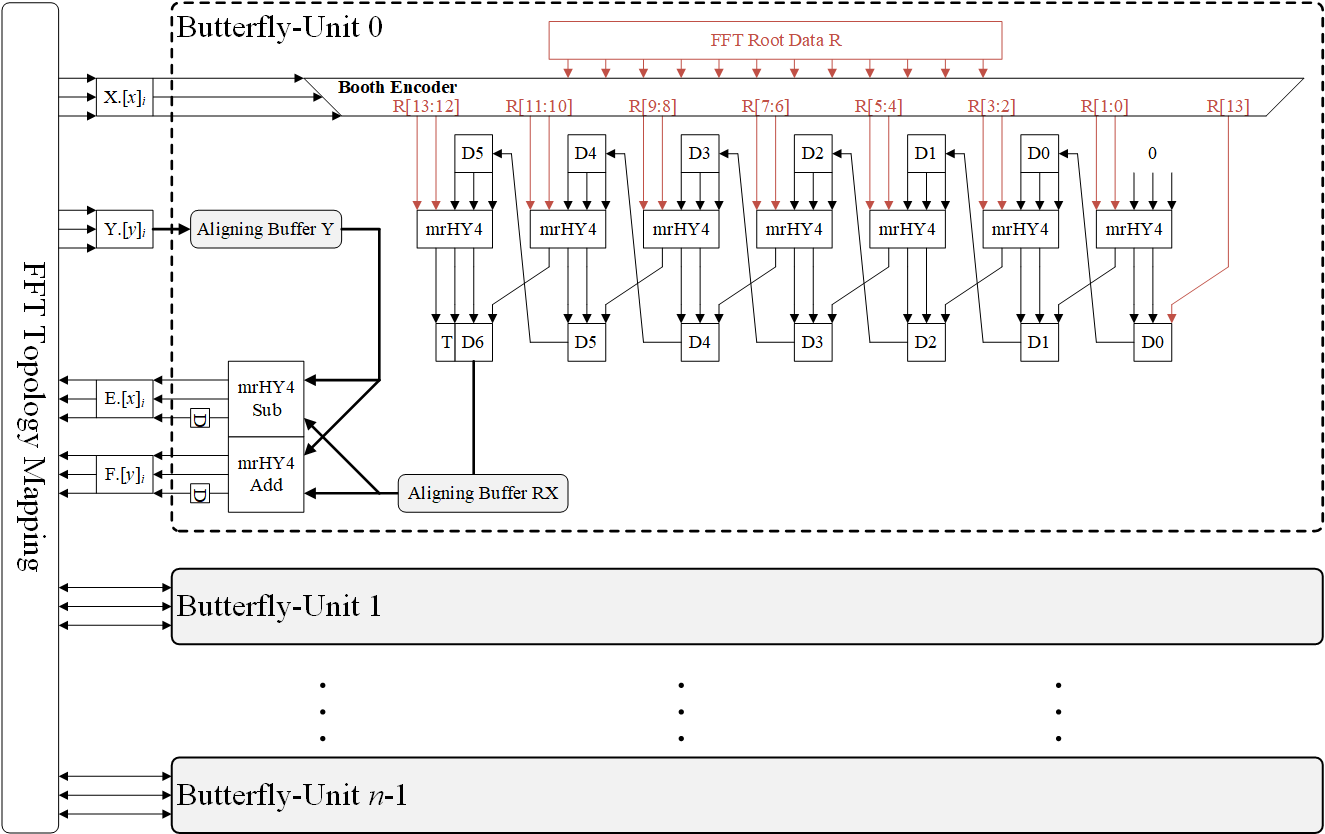
\includegraphics[width=0.6\textwidth]{figures/Float_Redundant_Butterfly_Unit.png}
        \caption{蝶形运算单元}
        \label{fig:Float-Redundant-Butterfly-Unit}
    \end{figure}
\end{center}

在这一过程中,两级运算流水执行,并无空闲等待时间,如下图任务流程图所示。
每级流水的执行时间与量化精度(即冗余量化位 $LEN$)有关,且乘法与加、减法所需执行周期均等于量化位数 $\mathrm{LEN}$。
对于一个$N=2^n$ 点的FFT,其共包含 $\log_2N$ 级别蝶形运算,故而系统工作的总周期数为:
\begin{equation*}
    (\log_2 N+1)\cdot \mathrm{LEN},\qquad \tag{C1}
\end{equation*}

Mapping 模块实现了如下图所示拓扑。得益于选用折叠的乘法和加法结构,
每个蝶形计算单元的面积已经尽可能地减小了,故而降低了多点数全并行蝶形单元的部署压力。
\begin{center}
    \begin{figure}[h!]
        \centering
        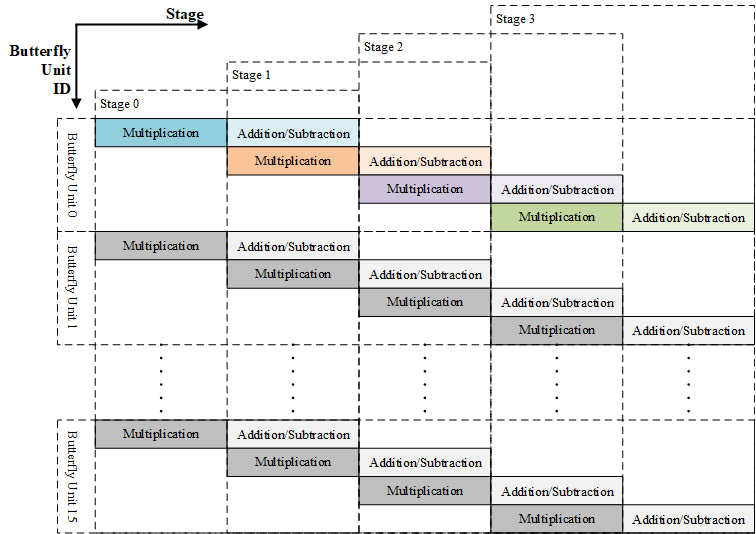
\includegraphics[width=0.5\textwidth]{figures/Pipeline.png}
        \caption{项目流水线示意图}
        \label{fig:Pipeline}
    \end{figure}
\end{center}

在我们的处理模块中,$N$ 个蝶形单元并行处理数据,它们的输出经过 Mapping 模块映射到其他蝶形单元的输入端,
结合流水化的运算流程,全自动地完成FFT的多级计算,
除了原根输入和 Reset 操作外,整个系统不包含状态机和控制逻辑,实现了自动化的流处理操作。

\subsection{\heiti{Booth 无进位乘法和 Karatsuba 快乘(Booth Multiplication Algorithms \& Karatsuba Multiplication)}}

本文选用了``基四最小冗余(Minimal Redundant Radix-4,mr4)''方案,
对于任意一个 $2n$ 二进制位的整数 $X\in\Z$,其mr4冗余表达式为:
\begin{eqnarray*}
    X=\sum_{i=0}^{n-1}[x]_i\cdot 4^i
\end{eqnarray*}

其中数位 $[x]_i\in\{-2,-1,0,1,2\}$,在计算机中 $[x]_i$ 由三个比特 $\{x_i^{-2},x_i^{+},x_i^{++}\}\in\{0,1\}^3$ 表示,即
\begin{eqnarray*}
    [x]_i=-2\cdot x_i^{-2}+x_i^{+}+x_i^{++}
\end{eqnarray*}

相较于传统的二进制补码表示法,mr4冗余表示具有以下三点优势:
\begin{itemize}
    \item   传统的存在进位传播的二进制加法在硬件实现时往往要考虑进位传播;
            而冗余示数法具有多映射的特点,即相同的 $X$ 具有多个不同的冗余表达式,
            利用这一特点,我们可以实现无``进位传播''的冗余加法,如图``基四最小冗余混合加法(mrHY4A)'',如下图\ref{fig:mrHY4A}。
            \begin{center}
                \begin{figure}[ht!]
                    \centering
                    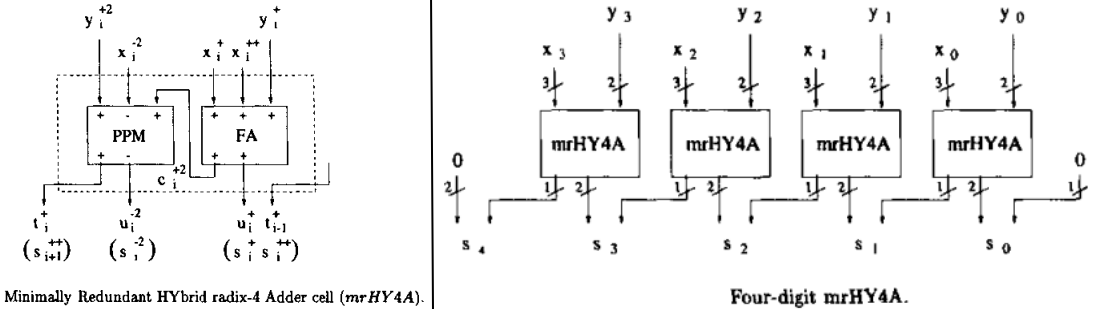
\includegraphics[width=0.8\textwidth]{figures/mrHY4A.png}
                    \caption{基四最小冗余混合加法(mrHY4A)}
                    \label{fig:mrHY4A}
                \end{figure}
            \end{center}
    \item   对于存在进位传播的传统二进制加法,其大端先入(MSB-first-in)
            折叠架构相较于小端先入(LSB-first-in)
            在硬件复杂度上具有天然的劣势;然而对于冗余表示,
            其大端和小端先入结构在硬件复杂度上几乎没有差别,如下图所示。
            \begin{center}
                \begin{figure}[ht!]
                    \centering
                    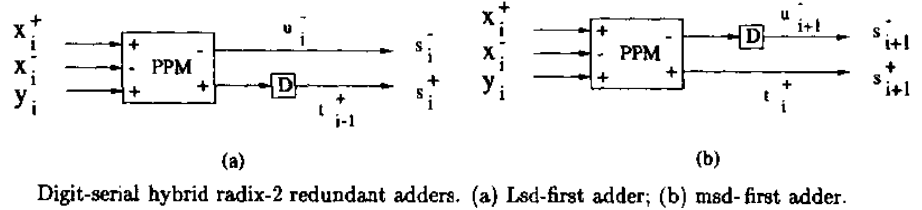
\includegraphics[width=0.8\textwidth]{figures/serial_mrHY4A.png}
                    \caption{Serial mrHY4A}
                    \label{fig:serial-mrHY4A}
                \end{figure}
            \end{center}
    \item   mr4 冗余表示不需要符号位,其所表示数字 $X$ 的符号蕴含在 
            $\{x_i^{-2},x_i^{+},x_i^{++}\}$ 的大小关系之中,这让我们避免了运算过程中的符号位扩展问题。
\end{itemize}

在浮点运算中,浮点加法的设计难度在于尾数的对齐。
因而相较于定点数加法,浮点数加法具有更高的硬件复杂度。
本文基于冗余mr4表示,针对浮点加法提出了一个大端先入的折叠计算模块。
如下图所示为量化精度为 $6$ 个数位($12$ 个二进制位)的冗余浮点加法运算过程,
为保持输出仍为6位的量化精度,该串行加法执行 $6$ 次,串行输出 $S=A+B$ 的每一个冗余数位。
其中,$B$ 的阶码比 $A$ 小3阶,故而在大端加法的前3个周期,只有数字 $A$ 所属移位寄存器移位输出。
在浮点数的串行加法中,大端先入是避免复杂对齐操作的关键,而冗余计算的大端先入串行加法具有和小端先入同等的复杂程度。
\begin{center}
    \begin{figure}[hb!]
        \centering
        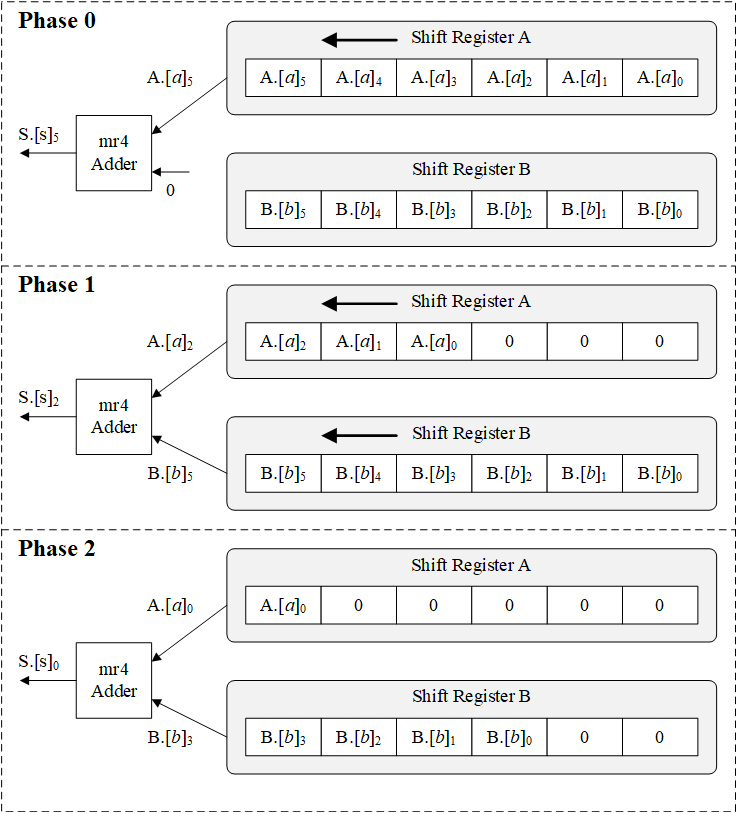
\includegraphics[width=0.55\textwidth]{figures/Float_Redundant_Adder.png}
        \caption{冗余浮点加法运算过程}
        \label{fig:Float-Redundant-Adder}
    \end{figure}
\end{center}

为配合大端先入的冗余浮点加法模块,本文继续设计了一款大端先入先出的串行冗余乘法单元,其主要电路结构入下图所示。
图中乘法器输入为FIR数据点 $X$ 和 FFT 单位根 $R$,其中在单次乘法过程中,$R$ 为固定输入,
而$X$ 所在的串行移位寄存器连接到 Booth 编码器(Booth Encoder)的输入端,完成对单位根 $R$ 的Booth编码,
编码输出作为当前输入与部分积 $D$ 累加。因为冗余加法不存在进位传播,故而 $D$ 的最高位 $D6$ 可以直接作为当前乘积的有效位而输出。
该结构迭代6次即可完成一次 $6$ 数位($12 \, \mathrm{bit}$ 精度)的乘法。
\begin{center}
    \begin{figure}[ht!]
        \centering
        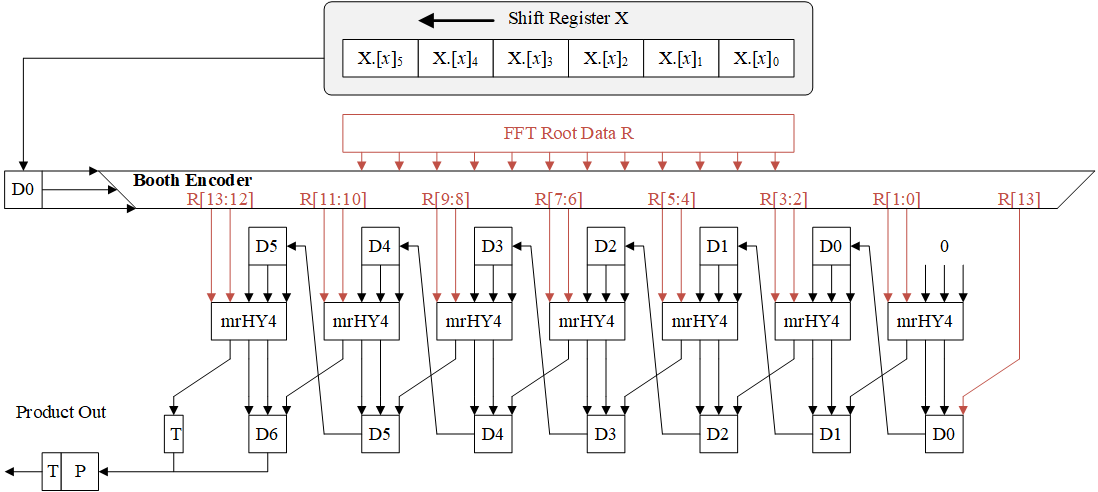
\includegraphics[width=0.6\textwidth]{figures/Redundant_Multiplier.png}
        \caption{冗余浮点乘法运算过程}
        \label{fig:Redundant-Multiplier}
    \end{figure}
\end{center}

\paragraph{\heiti{Karatsuba 快乘}}
以下对于高精度大整数乘法的 Karatsuba 算法简介摘录自 \href{https://oi-wiki.org/math/bignum/#karatsuba-%E4%B9%98%E6%B3%95}{OI Wiki:Karatsuba Algorithm}。

如果取高精度数字(必要时同时约化为大整数)的位数为 $n$,那么高精度—高精度竖式乘法需要花费 $\O(n^2)$ 的时间。
本节介绍一个时间复杂度更为优秀的算法,由前苏联(俄罗斯)数学家 Anatoly Karatsuba 提出,是一种分治算法。

考虑两个十进制大整数 $x$ 和 $y$,均包含 $n$ 个数码并可以有前导零。任取 $0 < m < n$,记
\begin{eqnarray*}
    \begin{aligned}
        x &= x_1 \cdot 10^m + x_0, \\
        y &= y_1 \cdot 10^m + y_0, \\
        x \cdot y &= z_2 \cdot 10^{2m} + z_1 \cdot 10^m + z_0,
    \end{aligned}
\end{eqnarray*}

其中 $x_0,y_0,z_0,z_1 < 10^m$。简单四则运算可得
\begin{eqnarray*}
    \begin{aligned}
        z_2 &= x_1 \cdot y_1, \\
        z_1 &= x_1 \cdot y_0 + x_0 \cdot y_1, \\
        z_0 &= x_0 \cdot y_0.
    \end{aligned}    
\end{eqnarray*}

继续观察(本质上使用分配律或 Wingoard 加速算法)将
\begin{eqnarray*}
    z_1 = (x_1 + x_0)(y_1 + y_0) - z_2 - z_0
\end{eqnarray*}

从而只要计算出 $(x_1+x_0), (y_1 + y_0)$ 再与 $z_2,z_0$ 相减即可求出 $z_1$。

因为普遍讲计算机上乘法的耗时要大于甚至远大于加法(尤其是数位越大的时候)。从而将乘法替换为
加法会大大降低算法的渐进时间复杂度。

上式实际上是 Karatsuba 算法的核心,它将长度为 $n$ 
的乘法问题转化为了 3 个长度更小的子问题。若令 
\begin{eqnarray*}
    m = \left\lceil \dfrac n 2 \right\rceil
\end{eqnarray*} 

记 Karatsuba 算法计算两个 $n$ 位整数乘法的耗时
为 $T(n)$,则有 
\begin{eqnarray*}
    T(n) = 3 \cdot T \left(\left\lceil \dfrac n 2 \right\rceil\right) + \O(n)
\end{eqnarray*}

由主定理可得 
\begin{eqnarray*}
    T(n) = \O (n^{\log_2 3}) \approx \O (n^{1.585})
\end{eqnarray*}

这相比于通常的大整数乘法的 $\O (n^2)$ 有数量级的减少。也回答了 20世纪 60年代 Kolmogorov 关于大整数乘法渐进时间复杂度是否
为 $\Omega(n^2) \approx \O (n^2)$ 的重大问题。

而 Anatoly Karatsuba 发明这个算法时年仅 23 岁,仅仅是在 Kolmogorov 陈述他关于任何大整数乘法算法的
时间复杂度趋于 $\O(n^2)$ 这一猜测一周后 Karatsuba 就完成了上述更快算法的构造。具体的历史信息可参考 
\href{https://en.wikipedia.org/wiki/Karatsuba_algorithm}{Wikipedia:Karatsuba Algorithm}。其中一段摘录如下

\begin{quote}
    In 1960, 
    Kolmogorov organized a seminar on mathematical problems in cybernetics 
    at the Moscow State University, where he stated the $\Omega (n^2)$ conjecture and other problems 
    in the complexity of computation. Within a week, Karatsuba, then a 23-year-old student, found an
     algorithm that multiplies two n-digit numbers in $\O (n^{\log_2 3})$ elementary steps, thus 
    disproving the conjecture. Kolmogorov was very excited about the discovery; 
    he communicated it at the next meeting of the seminar, which was then terminated. 
    Kolmogorov gave some lectures on the Karatsuba result at conferences all over the world 
    (see, for example, ``Proceedings of the International Congress of Mathematicians 1962'', 
    pp. 351–356, and also ``6 Lectures delivered at the International Congress of Mathematicians 
    in Stockholm, 1962'') and published the method in 1962, in the Proceedings of the USSR Academy 
    of Sciences. The article had been written by Kolmogorov and contained two results on 
    multiplication, Karatsuba's algorithm and a separate result by Yuri Ofman; it listed 
    \textquotedbl A. Karatsuba and Yu. Ofman\textquotedbl as the authors. Karatsuba only became aware of the paper 
    when he received the reprints from the publisher.
\end{quote}

更完整的第一手算法理论参考可见 Karatsuba 本人的综述 \cite{Karatsuba1995}。本项目使用其思想实现了针对滤波器乘法的版本如下,
主要集成了 Karatsuba 算法实现了多项式乘法和卷积,最后再处理所有的进位问题。具体信息参考源代码或附录。

\subsection{\heiti{量化感知中的混合精度量化(Mixed Precision Quantization)}}

此部分主要参考 \citetitle{Gholami2021} 的大量参考文献中实现的不同的量化感知技术。

\paragraph{\heiti{混合精度量化}}

选取最优的数据混合精度,硬件可以追求准确度与计算成本之间的平衡。

量化感知技术为硬件带来了效率提升。我们能够发现,在低精度计算模式下,量化感知技术可以让硬件计算速度完成提升。
但我们发现,对于一个元件而言,全部计算参数的低精度处理常常会带来元件工作准确度的大幅下降。
因此,为了保证元件工作的准确性,同时维持元件的高效运行,不同硬件采用不同的计算精度成为了合适的选择。
混合精度量化因此被提出,旨在研究对于某一固定硬件架构,应该选择什么样的低精度计算策略。

\begin{center}
    \begin{figure}[ht!]
        \centering
        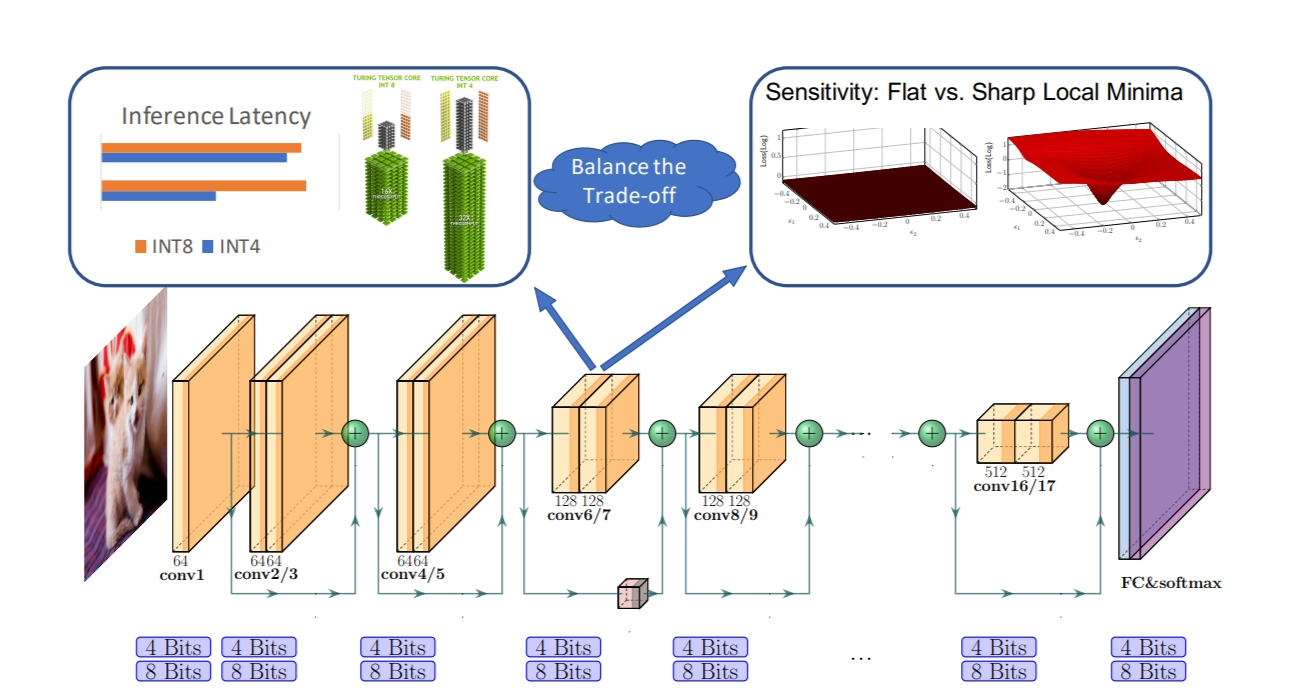
\includegraphics[scale = 0.5]{figures/multprecision.png}
        \caption{一种混合精度神经网络架构}
        \label{fig:multprecision}
    \end{figure}
\end{center}

如图\ref{fig:multprecision}所示,整个神经网络架构的各个卷积层分别选取了不同的参数精度,在不同参数精度的条件下分别进行训练。
在训练过程中挑选效果最优的精度组合,最终构成硬件结构的实际参数。

上述过程是混合精度量化的大体过程。对于混合精度量化模型的训练而言,通常有不同的训练方式。

在量化模型训练过程中,通常采用与全精度浮点模型不同的方式。如图\ref{fig:differentlpmethods}左表示的是浮点模型的训练方式。
浮点模型直接通过浮点数运算进行网络训练。而计算机在处理量化模型时一般采用模拟量化训练与完全量化训练两种方式,即图\ref{fig:differentlpmethods}剩余两部分的量化训练方法。


\begin{center}
    \begin{figure}[ht!]
        \centering
        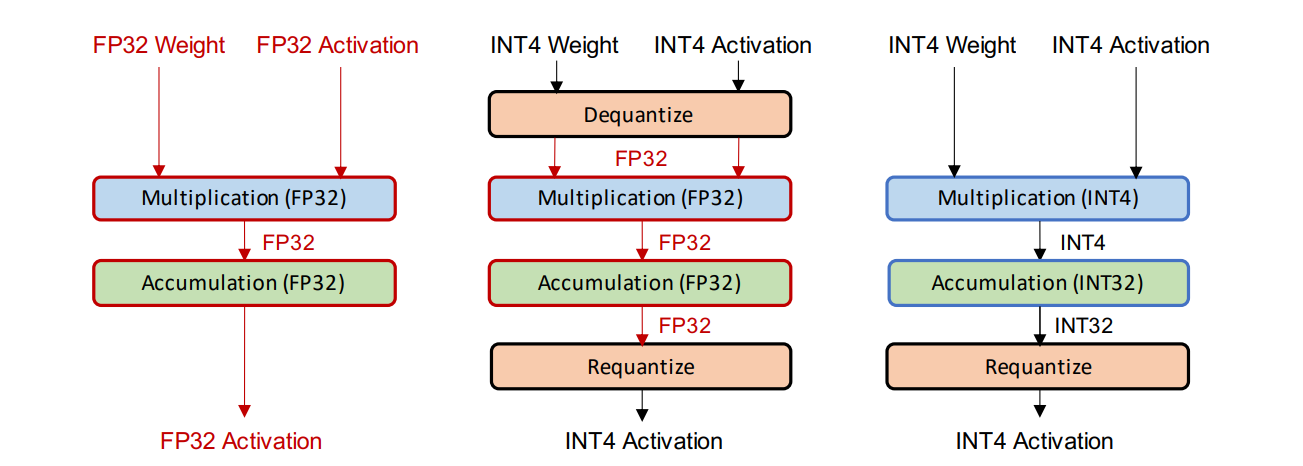
\includegraphics[scale = 0.5]{figures/differentLPmethods.png}
        \caption{量化神经网络的模型训练方法}
        \label{fig:differentlpmethods}
    \end{figure}
\end{center}


模拟训练量化的全部参数被储存在不同精度格式下,但在训练时首先通过计算将参数转化为浮点数,再利用浮点数的训练模式进行参数训练。
浮点数参数训练的优势在于其训练时非线性部分可以被有效近似,训练比较稳定。

完全训练量化则是根据低精度的数据格式的计算来进行模型训练。在低精度下,求导等运算的准确度会有所降低,可能会引入较大的计算误差。
因此,寻求更为有效的低精度近似计算方法是提高量化模型训练效率的重要方向之一。

上述两种量化训练方式各有优势与劣势,在不同的训练任务中需要根据侧重进行合适地选取。
量化感知的混合精度量化技术仍然具有提升潜力,更为有效的低精度计算方法将为混合量化模型的训练提供更加有效的提升。

\section{\heiti{实验数据及软硬件介绍}}

为了进行公平的比较,我们在 Xilinx Artix-7 FPGA平台上,
分别对 $64$、$128$ 和 $256$ 点的 FFT 硬件设计进行了实验,以探索速度和面积效率之间的不同权衡。
为了考虑 DSP 和 BRAM,我们使用 Slice 等效成本(SEC)作为面积评估的度量。
通过 $\mathrm{SEC=\# BRAM x 200+\# DSPsx 100+\# Slice}$ 来计算 SEC,即一个 DSP 块和一个 36
 Kb BRAM 分别等于 $102.4$ 和 $196.2$ 片。
面积效率指标则由面积时间积(ATP)评估,
计算为\# SEC $\times$ FFT 算法执行时间。
我们将所提出的高效 FFT 流处理器性能与近期内和``FIR''、``多项式乘法''、
``傅里叶变换''和``蝶形运算''等主题相关的硬件工作做对比。
受益于我们所采用的冗余计算方案,
即使在高并行度的执行环境下,
我们的设计仍然可以跑到 $200$ Mhz、$177$ Mhz和 $162$ MHz。
为与所引工作进行公平比较,我们针对 $N=256$ 点的 FFT 做了实现,
其 ATP 评估结果为 $1813.7$,位列相关工作最优。
此外,为充分论证设计在不同并行度下的执行性能和面积、速度权衡,我们也针对 $N=64$ 以及 $128$ 做了实现,以供参考。
基于实现结果,我们推荐使用 $N=32\sim 128$ 的参数来加速 FIR 应用问题,以取得最佳的加速效果。

\section{实验结果及主要结论}

\subsection{主要测试结果}


\subsection{结论}

实现性能 $40 \% $ 的提升的结论。


\section{总结及展望}


\section*{附录}

\phantomsection
\addcontentsline{toc}{section}{附录}

这是附录文件。

The color of links can be changed to your liking using:

{\small\verb!\hypersetup{urlcolor=red}!}, or

{\small\verb!\hypersetup{citecolor=green}!}, or

{\small\verb!\hypersetup{allcolor=blue}!}.

\noindent If you want to completely hide the links, you can use:

{\small\verb!\hypersetup{allcolors=.}!}, or even better: 

{\small\verb!\hypersetup{hidelinks}!}.

\noindent If you want to have obvious links in the PDF but not the printed text, use:

{\small\verb!\hypersetup{colorlinks=false}!}.

\newpage
\phantomsection
\addcontentsline{toc}{section}{\heiti{参考文献}}
\printbibliography[title={\heiti{参考文献}}]


\end{document}
